%%%%%%%%%%%%%%%%%%%%%%%%%%%%%%%%%%%%%%%%%
% University/School Laboratory Report
% LaTeX Template
% Version 3.1 (25/3/14)
%
% This template has been downloaded from:
% http://www.LaTeXTemplates.com
%
% Original author:
% Linux and Unix Users Group at Virginia Tech Wiki 
% (https://vtluug.org/wiki/Example_LaTeX_chem_lab_report)
%
% License:
% CC BY-NC-SA 3.0 (http://creativecommons.org/licenses/by-nc-sa/3.0/)
%
%%%%%%%%%%%%%%%%%%%%%%%%%%%%%%%%%%%%%%%%%

%----------------------------------------------------------------------------------------
%	PACKAGES AND DOCUMENT CONFIGURATIONS
%----------------------------------------------------------------------------------------

\documentclass{article}

\usepackage[version=3]{mhchem} % Package for chemical equation typesetting
\usepackage{siunitx} % Provides the \SI{}{} and \si{} command for typesetting SI units
\usepackage{graphicx} % Required for the inclusion of images
\usepackage{natbib} % Required to change bibliography style to APA
\usepackage{amsmath} % Required for some math elements 
\usepackage[applemac]{inputenc}

\setlength\parindent{0pt} % Removes all indentation from paragraphs

\renewcommand{\labelenumi}{\alph{enumi}.} % Make numbering in the enumerate environment by letter rather than number (e.g. section 6)

%\usepackage{times} % Uncomment to use the Times New Roman font

%----------------------------------------------------------------------------------------
%	DOCUMENT INFORMATION
%----------------------------------------------------------------------------------------

\title{Simulazione e Ottimizzazione di un Impianto di Teleriscaldamento da Fonte Geotermica } % Title

\author{Marco \textsc{Becattini}} % Author name

\date{} % Date for the report

\begin{document}

\maketitle % Insert the title, author and date

\begin{center}
\begin{tabular}{l r}
%Date Performed: & January 1, 2012 \\ % Date the experiment was performed
Instructors: & A. Vicino,  A. Giannitrapani,  S. Paoletti \\ % Partner names
Partner: & R. Parri % Instructor/supervisor
\end{tabular}
\end{center}

% If you wish to include an abstract, uncomment the lines below
% \begin{abstract}
% Abstract text
% \end{abstract}

%----------------------------------------------------------------------------------------
%	SECTION 1
%----------------------------------------------------------------------------------------

\section{Obiettivo}

In un impianto di teleriscaldamento alimentato da fonte di calore geotermica gli unici costi di gestione dell'impianto derivano dalla potenza data alle pompe per il pompaggio delle acque di circolazione. Le stazioni di pompaggio lavorano a regime variabile e per un ottimizzazione del sistema, bisogna far si che le pompe lavorino in condizioni di  buon rendimento e non si sprechi energia di pompaggio. Se nella rete di distribuzione non vi sono regolazioni (assenti le centraline d'utenza), tutta la portata circola nei primi scambiatori e per alimentare gli ultimi si deve pompare un maggior quantitativo di acqua, inoltre, le temperature di ritorno delle prime utenze saranno pi\`u  alte. Le centraline di utenza risultano essere un elemento fondamentale per la regolazione e l'ottimizzazione di un impianto di teleriscaldamento in quanto dovrebbero limitare la portata dell'utenza allo stretto indispensabile e dovrebbero limitare al massimo la temperatura di ritorno. Pi\`u  le temperature di ritorno sono basse maggiore sar\`a  il rendimento.

% If you have more than one objective, uncomment the below:
%\begin{description}
%\item[First Objective] \hfill \\
%Objective 1 text
%\item[Second Objective] \hfill \\
%Objective 2 text
%\end{description}

 
%----------------------------------------------------------------------------------------
%	SECTION 2
%----------------------------------------------------------------------------------------

\section{Descrizione Impianto di Teleriscaldamento}

\textbf{Teleriscaldamento}: sistema di riscaldamento a distanza di un quartiere o di una citt\`a  che utilizza il calore prodotto da una centrale termica, da un impianto di cogenerazione o come nel nostro caso da sorgente geotermica. Il calore viene distribuitagli edifici tramite una rete di tubazioni in cui fluisce l'acqua calda.

Il teleriscaldamento \`e una soluzione per la produzione di acqua igienico sanitaria e il riscaldamento degli edifici residenziali e commerciali.\\

Dalla centrale termica si produce acqua calda e viene portata dalla rete di distribuzione primaria fino ad una centrale di scambio. In quest'ultima si decide a che temperatura mandare l'acqua nel circuito secondario e con quale portata. L'acqua quindi viene mandata alle utenze, ognuna delle quali disporr\`a  di piccole sottocentrali di scambio costituite da scambiatori di calore, che permettono di realizzare lo scambio termico tra il fluido termovettore e l'acqua del circuito delle utenze, senza che vi sia miscelazione tra i due fluidi semplificando la progettazione dell'intera rete. Dopo che nell'edificio \`e stato trasferito il calore necessario per riscaldare gli ambienti e per produrre acqua calda sanitaria. L'acqua, ormai raffreddata, ritorna in centrale per essere di nuovo riscaldata. L'impianto di distribuzione interno agli edifici allacciati alla rete resta inalterato e lo scambiatore di calore sostituisce la caldaia convenzionale. 

Gli impianti di teleriscaldamento geotermico utilizzano fluido non idoneo (oppure in alcuni casi idoneo) alla produzione di energia elettrica. Il funzionamento \`e schematizzato in figura  \ref{fig:schema1}.

\begin{figure}[h]
\begin{center}
\includegraphics[width=1.15\textwidth]{schema_impianto} % Include the image placeholder.png
\caption{Schema impianto di teleriscaldamento}
\label{fig:schema1}
\end{center}
\end{figure}


%----------------------------------------------------------------------------------------
%	SECTION 3
%----------------------------------------------------------------------------------------

\section{Sistema scambiatore utenza}
\subsection{Scambiatore}
Gli scambiatori di calore sono delle apparecchiature nelle quali si ha trasmissione del calore da un fluido ad un altro. Le variabili in gioco sono elencate in seguito:

\begin{itemize}
\item[] $G_p$ = portata del circuito primario
\item[]$G_u$ = portata del circuito secondario (parte utenza)
\item[]$c_s$ = calore specifico dell'acqua
\item[]$T_i$ = Temperatura di ingresso scambiatore dalla parte del circuito primario (acqua calda)
\item[]$T_o$ = Temperatura in uscita dallo scambiatore dalla parte del circuito primario (acqua fredda)
\item[]$t_i$ = Temperatura di ingresso scambiatore dalla parte del circuito secondario (acqua fredda)
\item[]$t_o$ = Temperatura in uscita dallo scambiatore dalla parte del circuito secondario (acqua calda)
\end{itemize}

\begin{figure}[h]
\begin{center}
\includegraphics[width=1.05\textwidth]{scambiatore} % Include the image placeholder.png
\caption{Schema di uno scambiatore all'interno di un utenza}
\label{fig:scamb}
\end{center}
\end{figure}

Applicando le equazioni di bilancio di massa e di energia al fluido caldo ed al fluido freddo si ottengono le seguenti formule per il calcolo della potenza termica globale, $W_t$. Nello studio degli scambiatori di calore \`e  utile riferirsi alla cosiddetta portata termica (oraria), $C$, data dal prodotto tra la portata massica ed il calore specifico:
\begin{equation}
C_p=G_p c_s  \ \ \ ; \ \ \ C_u=G_u c_s
\end{equation}
In tal caso le due equazioni di bilancio  possono scriversi nella seguente forma:
\begin{equation}
W_t=C_p(T_i - T_o) \ \ \ ; \ \ \ W_t=C_u(t_o - t_i)
\end{equation}
A queste due equazioni di bilancio energetico, si pu\`o  associare una equazione di scambio termico; quest'ultima associa la potenza termica scambiata tra i due fluidi alle temperature di ingresso e/o di uscita, alle portate, al coefficiente di scambio termico globale ed all?area di scambio. Questa equazione deriva dal metodo della media logaritmica delle differenze di temperatura (o MLDT) dove  la potenza termica scambiata tra i due fluidi viene legata alla differenza di temperatura tra il fluido caldo ed il fluido freddo dalla seguente relazione:
\begin{equation}
W_t=\alpha S \Delta T_{ml} \\
\end{equation}
\begin{center}
 $\Delta T_{ml} = \frac{(\Delta T_1)-(\Delta T_2)}{log\left( \frac{\Delta T_1}{\Delta T_2} \right)}$ \\
 \end{center}
 \begin{center}
 Se scambiatore in corrente : $ \Delta T_1 = T_i - t_i $  \ \ ; \ \ $ \Delta T_2 = T_o - t_o $  \\
 
 Se scambiatore in controcorrente : $ \Delta T_1 = T_i - t_o $  \ \ ; \ \ $ \Delta T_2 = T_o - t_i $ 
\end{center}
dove $S$ \`e  la superficie attraverso cui avviene lo scambio ed $\alpha$ \`e  il cosiddetto coefficiente di scambio termico globale o conduttanza termica unitaria. 

In figura \ref{fig:andamento} \`e  possibile vedere l'andamento delle temperature negli scambiatori in corrente (a) e in controcorrente (b).
\begin{figure}[h]
\begin{center}
\includegraphics[width=0.95\textwidth]{grafico_scambiatore} % Include the image placeholder.png
\caption{Andamento delle temperature negli scambiatori }
\label{fig:andamento}
\end{center}
\end{figure}

\subsection{Utenza}
Esiste ovviamente una formula matematica che consente un calcolo approssimativo del fabbisogno termico. Bisogna per\`o  tenere presente che \`e  un risultato indicativo e, appunto, approssimativo, poich\'e ci sono moltissime variabili che possono incidere sul reale fabbisogno dell'abitazione, alcune delle quali difficilmente quantificabili. 

Il calcolo matematico fornisce il totale delle Kilocalorie necessarie a scaldare l'abitazione utilizzando come dati di partenza
\begin{itemize}
\item  il totale dei metri cubi da scaldare,
\item    un coefficiente termico che indica le calorie necessarie per metro cubo e che pu\`o  oscillare tra un valore che va da 30 a 40 $\frac{Kcal}{m^3}$, a seconda delle condizioni termiche dell'abitazione.
\end{itemize}

Nei futuri calcoli considereremo  un appartamento di 100 $m^2$ con soffitti non pi\`u  alti di 3 $m$ e coefficiente termico di 30 $\frac{Kcal}{m^3}$. Il fabbisogno termico di risulter\`a  di circa 9000 $Kcal$ (10440 $W$).

Questo valore ci da un indice di quanta energia i radiatori dovranno fornire alla casa per scaldarla.

\subsubsection{Radiatori}
I radiatori (figura \ref{fig:radiatore}) sono gli elementi all'interno dell'utenza che trasferiscono calore all'ambiente per scaldarlo. 
\begin{figure}[h]
\begin{center}
\includegraphics[width=0.75\textwidth]{schema_radiatore} % Include the image placeholder.png
\caption{Schematizzazione di un radiatore}
\label{fig:radiatore}
\end{center}
\end{figure}
La potenza emessa da un corpo scaldante dipende dalla sua temperatura media tra il fluido caldo in ingresso al radiatore e quello freddo in uscita dalla seguente relazione:
\begin{equation}
P_{radiatore} = Km(\frac{t_o + t_i}{2} - \Theta_{amb})^n
\end{equation}
con Km e n coefficienti che dipendono dal tipo di radiatore in uso costanti. \\

Un'altra considerazione da fare riguarda il comportamento dei radiatori in termini di potenza emessa al variare della portata. In figura \ref{fig:portata} si nota gli andamenti delle potenze in funzione delle temperature di mandata e ritorno dal radiatore con portate diverse. Diminuendo la portata le curve di temperatura $t_o$ e $t_i$ si aprono come un ventaglio man mano che la portata diminuisce e viceversa.

\begin{figure}[h]
\begin{center}
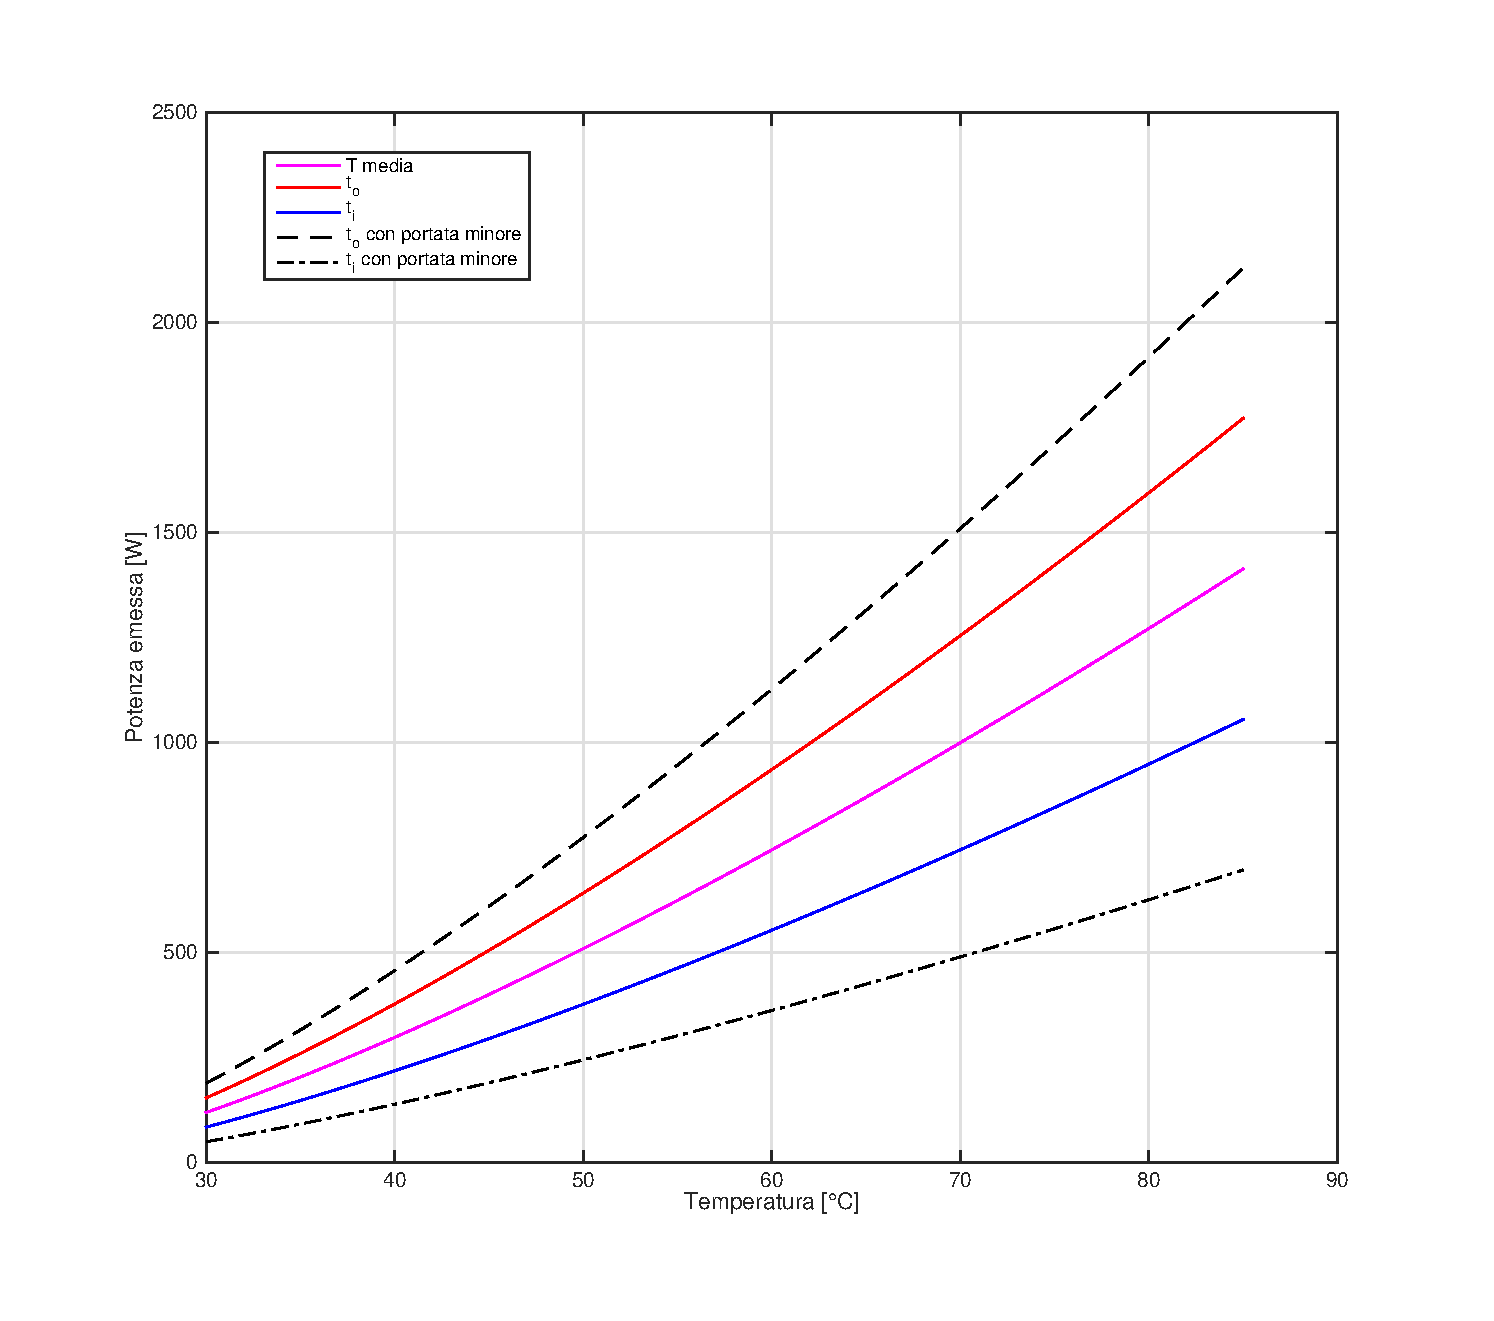
\includegraphics[width=0.75\textwidth]{grafico_scambio_radiatore} % Include the image placeholder.png
\caption{Grafico andamento della potenza scambiata in funzione delle temperature e portate diverse}
\label{fig:portata}
\end{center}
\end{figure}

E' possibile ottenere  le stesse potenze termiche con due portate diverse facendo variare la differenza di temperatura tra fluido caldo e freddo, e di conseguenza alzando o abbassando le temperature di mandata e ritorno dei radiatori. Diminuendo la portata il radiatore scambia di pi\`u  e ci\`o  comporta una riduzione dell'acqua di ritorno dal radiatore. Se per\`o  la temperatura in mandata rimane la stessa avremo una potenza scambiata dal radiatore minore in quanto si \`e  abbassata la temperatura media del fluido all'interno del radiatore (figura \ref{fig:radiatore1}).

\begin{figure}[h]
\begin{center}
\includegraphics[width=0.75\textwidth]{Tcostante} % Include the image placeholder.png
\caption{Schema di funzionamento radiatore con temperatura di mandata costante e portate variabili}
\label{fig:radiatore1}
\end{center}
\end{figure}

Se vogliamo ottenere una potenza maggiore  dovremmo aumentare la temperatura in mandata in modo da far aumentare la temperatura media (figura \ref{fig:radiatore2}))

\begin{figure}[h]
\begin{center}
\includegraphics[width=0.75\textwidth]{Tvariabile} % Include the image placeholder.png
\caption{Schema di funzionamento radiatore con temperatura di mandata variabile al fine di ottenere potenze di scambio uguali anche se le portate sono diverse}
\label{fig:radiatore2}
\end{center}
\end{figure}
\clearpage
\subsection{Simulazione}
Andremo in seguito a simulare il sistema scambiatore utenza per capire il comportamento delle temperature e portate al variare di alcuni parametri (figura \ref{fig:scamb_utenza}). 

\begin{figure}[h]
\begin{center}
\includegraphics[width=0.95\textwidth]{sistema_scamb_casa} % Include the image placeholder.png
\caption{rappresentazione schematica sistema scambiatore e utenza}
\label{fig:scamb_utenza}
\end{center}
\end{figure}

Andremo quindi a costruirci un sistema dinamico dove la nostra variabile di stato \`e  la temperatura ambiente che da ora in avanti verr\`a  indicata con $\Theta_{amb}$. Il nostro sistema sar\`a  descritto dalla seguente relazione:
\begin{center}
$MC \Theta'_{amb} = W_{scambiata} - W_{dispersa}$ 
\end{center}
\begin{equation}
K_m(\frac{t_o + t_i}{2} - \Theta_{amb})^n - K( \Theta_{amb} - \Theta_{est}) = MC \Theta'_{amb}
\end{equation}
\begin{itemize}
\item[] $K_m$ = costante $K_m$
\item[]$n$ = esponente
\item[]$K$ = coefficiente di dispersione termica
\item[]$\Theta_{amb}$ = Temperatura ambiente (variabile di stato)
\item[]$\Theta_{est}$ = Temperatura esterna
\item[]$M$ = Massa dell'utenza
\item[]$C$ = capacit\`a  termica
\end{itemize}

Le variabili note sono: $G_u, T_i, t_o$\\
Le variabili incognite sono: $G_p, T_o, t_i$\\

Le incognite si possono ricavare da un sistema tre equazioni tre incognite. Facendo l'assunzione che la potenza termica scambiata dallo scambiatore \`e  uguale alla potenza scambiata dai radiatori otteniamo il seguente sistema di equazioni:
\begin{equation}
\left \{
\begin{array}{rl}
K_m(\frac{t_o + t_i}{2} - \Theta_{amb})^n = C_u(t_o - t_i)\\
\\
C_p(T_i - T_o) = C_u(t_o - t_i)\\
\\
C_u(t_o - t_i) = \alpha S \frac{(T_i - t_o)-(T_o - t_i )}{log\left( \frac{T_i - t_o}{T_o - t_i } \right)}\\
\end{array}
\right.
\end{equation}

Il  lavoro successivo sar\`a  quello di inserire un riferimento per la temperatura ambiente e regolare il sistema in modo da mantenere la temperatura desiderata all'interno dell'utenza.
I modi per regolare il calore fornito all'utenza sono:
\begin{itemize}
\item agire sulla valvola di laminazione regolando la portata sul circuito primario e quindi la temperatura in mandata dell'acqua.
\item con la premessa di avere pompe a regime variabile, regolare la portata sul secondario (utenza).
\end{itemize}
L'obiettivo principale come detto in precedenza sar\`a  quello di trovare un metodo che permetta di avere la temperatura di ritorno alla centrale di scambio pi\`u  bassa possibile in modo da aumentare il rendimento dell'impianto e diminuire gli sprechi.\\

Per aumentare l'efficienza e per ridurre al massimo gli sprechi si \`e  pensato di introdurre un ulteriore regolazione. Solitamente l'utenza regola con termostato e il comportamento dell'utenza nei riguardi della regolazione di quest'ultimo dipende molto dalla modalit\`a  di fatturazione; infatti con fatturazione a forfait la regolazione del termostato sar\`a  sempre pi\`u  vicina ai 30 che ai 20 gradi. Questo comporta che il carico termico del sistema di teleriscaldamento \`e sempre vicino al massimo invernale. Un metodo pensato per cautelarsi rispetto a  condizioni di cattiva gestione della regolazione della temperatura all'interno delle abitazioni \`e  quella di regolare la temperatura massima in mandata nell'utenza in funzione della temperatura esterna (figura \ref{fig:tem} ).

\begin{figure}[h]
\begin{center}
\includegraphics[width=0.95\textwidth]{temperature} % Include the image placeholder.png
\caption{rappresentazione schematica sistema scambiatore e utenza}
\label{fig:tem}
\end{center}
\end{figure}

Il fabbisogno energetico  aumenta al diminuire  della temperatura esterna e viceversa. Si vuole procedere in questo modo perch� pi\`u  le temperature di ritorno sono basse pi\`u  il rendimento \`e  elevato ed utilizzando una regolazione di questo tipo nello scambiatore di utenza, si potrebbero avere temperature di ritorno tanto pi\`u  basse tanto \`e  minore il carico termico richiesto.
\clearpage
\section{ToDo}
Tramite l'uso di matlab andremo a simulare tre diversi scenari:
\begin{enumerate}
\item[1.] sistema scambiatore utenza senza alcun tipo di regolazione
\item[2.] sistema scambiatore utenza con regolazione fissa , dipendente dalla temperatura esterna (climatica): si imposta una temperatura in mandata $t_o$ sul secondario in funzione della temperatura esterna (regolare la temperatura in mandata implica regolare la portata sul primario)  
\item[3.] sistema scambiatore utenza con regolazione variabile in funzione della temperatura ambiente desiderata: si tratta di implementare un controllore MPC che ottimizza la temperatura di ritorno dell'acqua dati una funzione di costo e dei vincoli.
\end{enumerate}

\section{Risultati della simulazione}
\subsection{Potenze scambiate e temperature al variare delle portate}
I primi risultati ottenuti durante la simulazione riguardano l'andamento delle temperature e della potenza termica scambiata al variare delle portate.

\textbf{Porata sul primario $G_p$ variabile e portata sul secondario $G_u$ costante}: Maggiore \`e la portata sul primario maggiore \`e la potenza scambiata dallo scambiatore ed inoltre la temperatura di ritorno $T_o$ subisce un innalzamento e viceversa.

\textbf{Porata sul primario $G_p$ costante e portata sul secondario $G_u$ variabile}:Maggiore \`e la portata sul secondario minore risulta a differenza di temperatura tra $t_o$ e $t_i$ e viceversa. Il risultato pi\`u significativo ci mostra che variando la portata sul secondario, variano le temperature $t_o$ e $t_i$ ma variano in modo tale che la loro temperatura media ($\frac{t_o + t_i}{2}$ ) rimane costante come anche la temperatura di ritorno del primario $T_o$, visibile in figura \ref{fig:scambiatore_garico_temperature}.

\begin{figure}[h]
\begin{center}
\includegraphics[width=0.95\textwidth]{scambiatore_garico_temperature} % Include the image placeholder.png
\caption{rappresentazione schematica della variazione delle temperature al variare della portata sul secondario}
\label{fig:scambiatore_garico_temperature}
\end{center}
\end{figure}

In conclusione possiamo affermare che la potenza scambiata e la temperatura di ritorno $T_o$ dipende solamente dalla portata in mandata sul primario.\\

 La regolazione che dovremo implementare dovr\`a essere fatta sulla portata del primario in modo da limitare il ritorno di temperatura al minimo possibile ma tale da garantire la temperatura ambiente che \`e stata settata nel termostato. 

\section{Ulteriori considerazioni}
La portata delle pompe del circuito che porta l'acqua alle utenze non deve mettere in crisi le ultime abitazioni (la portata nelle prime utenze sar\`a  maggiore che nelle ultime). Se delle centraline di utenza regolassero le portate in ingresso agli scambiatori (utilizzando solamente quella strettamente necessaria) si ridurrebbe il problema. Si potrebbe controllare la portata dell'intero circuito con un sensore posizionato nell'ultima utenza dell'impianto per gestire la portata delle pompe.\\

Per regolare la portata sul circuito primario (dalla fonte geotermica alla centrale di scambio) si vorrebbe implementare un controllo. Nella centrale di scambio vi sono delle valvole che regolano la portata in modo da avere nel circuito nelle utenze una certa temperatura in mandata fissata. Ridurre la portata con una valvola di laminazione (se si vede la valvola come una resistenza variabile) vuol dire che si aumenta la resistenza del circuito con conseguente dispersione di energia (figure \ref{fig:resistenza}).
\begin{figure}[h]
\begin{center}
\includegraphics[width=0.85\textwidth]{resistenza} % Include the image placeholder.png
\caption{perdita sulla valvola di laminazione con regolazione a pressione costante}
\label{fig:resistenza}
\end{center}
\end{figure}
Quindi la migliore regolazione  delle pompe sarebbe con il segnale che regola la valvola in ingresso allo scambiatore. (problema da valutare \`e  inviare il segnale a qualche km di distanza).
\end{document}
